\let\textcircled=\pgftextcircled
\chapter{Modelling the effect of actuator-like behavior in dielectric elastomer generators}
\label{chap:1}

\initial{T}his chapter is based on the paper ''Modelling the effect of actuator-like behavior in dielectric elastomer generators``, published in the Volume 107 of Applied Physics Letters in 2015.



\section{INTRODUCTION}
\label{sec:intro}  % \label{} allows reference to this section

Dielectric elastomer generators (DEGs) are an emerging technology to harvest energy from the environment. Dielectric elastomers (DEs) consist of a layer of an elastic dielectric sandwiched between flexible electrodes, together acting as a variable capacitor\cite{RN226}. DEGs' technological appeal comes from their low cost, low weight and high energy density\cite{RN19}, making them a promising potential alternative to other electromechanical conversion technologies. Several applications have already been proposed, from energy scavenging to generation, converting energy from human motion, wind, or waves, and even heat to electricity\cite{RN19,RN18,MistralHMotion2008,RN166,RN194}.

To perform the electromechanical conversion, DEGs need a well timed process of charging and discharging, such that when the DEG relaxes from any induced deformation, the mechanical restoration forces due to the shape change performs work against the electrostatic forces of the charges stored in its structure. Thus, well timed charge is necessary to explore the full capacitance change and maximize energy conversion. Ideally, to guarantee maximum energy output, the DEG should finish charging before it reaches its maximum capacitance and cease discharging at minimum capacitance\cite{RN85}.

Despite their potential, practical implementation of DEGs still present issues, such as the need to charge the material to perform the energy conversion process. Although passive self-priming circuits (SPCs)\cite{spc1} and naturally polarized materials (such as electrets\cite{RN228}) have been employed as an alternative to manage charging, they do not necessarily allow the material to perform optimal harvesting cycles\cite{RN85}. Self-priming circuits need at least an initial charge to be supplied and will only present significant energy output after further cycles. Moreover, they are dependent on the capacitance swing to provide boost and may even yield voltage reduction if the capacitance change is too low\cite{spcpatrin,RN696}. Electrets have been used to polarize DEGs effectively, providing a permanent voltage source, but the energy density achieved by the systems is still low compared to active charging, when the DEG is charged through a power supply or similar in a well timed manner\cite{RN228,RN85}. In addition, electrets are not naturally soft and require extra design complexity to be implemented.

When looking for an upscale to optimise energy generation, additional sensors are required in order to detect states of maximal and minimal capacitance, which increase the cost and complexity of DEG system. Capacitance sensors based on charge measurements are typically more complicated than standard voltage and current sensors, since they are generally based on indirect measurement methods. In addition, the orders of magnitude of voltage (kV) and capacitance (nF) involved in typical DEG applications, and the parasitic leakage that exists in the material, further complicate the design of DEG capacitance sensors.

In this paper, we present a new method for charge management that integrates self-sensing capabilities into a DEG cycle. The method applies a straightforward algorithm to determine the moment of desired charge/discharge for a chosen cycle; it is robust to noise, and does not require knowledge of forcing parameters (frequency or amplitude).

\section{Self-sensing}
\subsection{DEG cycle and hardware}

In order to manage charge in the DEG, we first integrated existing self-sensing techniques, usually associated with dielectric elastomer actuators (DEAs), into the DEG. Several self-sensing methods have already been proposed for DEAs\cite{RN702}, some of which require the use of special hardware\cite{hoffstadtSS}, while others rely on strong post-processing\cite{GisbySS}. All of them require a sensing signal, usually a high frequency oscillatory voltage, to be superimposed over the slower actuation high voltage signal required by the DEA. The high-frequency sensing signal allows to increase the current absorbed by the device. In fact, the high-pass behavior of a DE makes the current resulting from typical low-frequency actuation too low to be accurately measured. On the other hand, the oscillatory signal does not produce actuation since it is usually beyond the mechanical bandwidth of the actuator. In order to  self-sense in a DEA, a simple circuit composed of a power supply directly attached to the DEA is enough. However, DEGs are integrated into a more complex circuit topology; due to the need for charge and discharge in every cycle, DEGs typically cycle through at least three circuit conditions:
\begin{enumerate}
\item the \emph{charging phase}, when the DEG is connected to a higher potential (e.g., a power supply) and current flows into it,
\item open-circuit, 
\item the \emph{discharging phase}, when the DEG is connected to a lower potential (e.g., a capacitor)  and current flows from it.
\end{enumerate}
We can only directly apply the self-sensing methods developed for DEAs to the charging phase, when a controlled power supply determines the voltage through the DEG. For the remaining phases, we must look for alternatives that will allow us to estimate the DEG's capacitance consistently.

In order to develop our method, we first defined the DEG circuit, and the energy harvesting cycle to be used. We chose a classic circuit topology for experimental work using DEGs, with two switches that allow the DEG to be connected to a power supply (S1) or to a load (S2) where it can discharge, as shown in \ref{fig:circuit}.
   \begin{figure}[htb]
   \begin{center}
   \begin{tabular}{c} %% tabular useful for creating an array of images 
   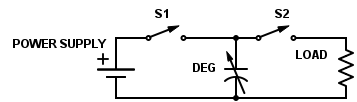
\includegraphics[scale=1.0]{\fig05\circuit.png}
   \end{tabular}
   \end{center}
   \caption[example] 
%>>>> use \label inside caption to get Fig. number with \ref{}
   { \label{fig:circuit} 
DEG circuit: S1 allows the DEG to charge under constant voltage, while S2 discharges the DEG through a constant load.}
   \end{figure} 

We then chose a cycle as described in \cref{fig:cycle}\cite{Zanini2017Frequency-domainGenerators} that consists of three phases:
\begin{enumerate}
\item stretch the DEG under constant voltage: charges flow to it as its capacitance increases,
\item allow the DEG to relax in open-circuit condition, keeping the charge level constant,
\item discharge (partially) the DEG until the charge reaches the same level as the start of the stretch phase.
\end{enumerate}
\begin{figure} [ht]
   \begin{center}
   \begin{tabular}{c} %% tabular useful for creating an array of images 
   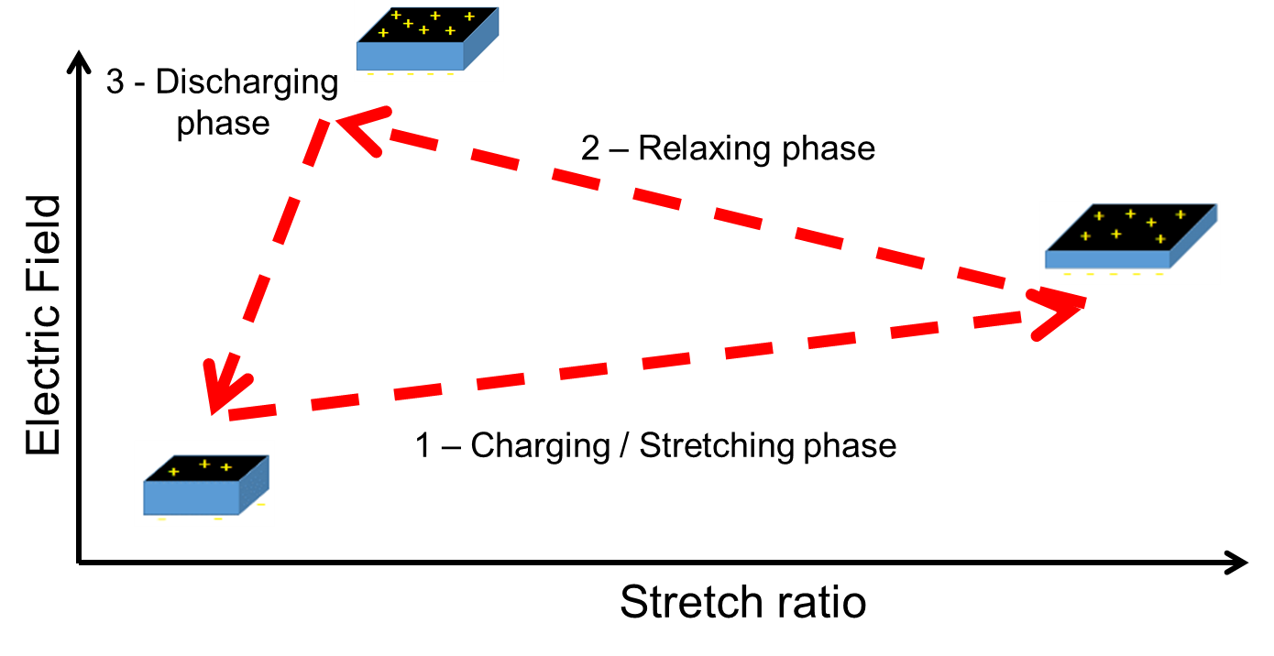
\includegraphics[height=5cm]{ExS_Cycle.png}
   \end{tabular}
   \end{center}
   \caption[example] 
%>>>> use \label inside caption to get Fig. number with \ref{}
   { \label{fig:cycle} 
Schematic illustration of the three phases of the DEG cycle.}
   \end{figure} 
Such cycle allows us to directly charge the DEG during its stretch phase, and simultaneously to apply an additional sensing signal from the power supply, and hence to use existing self-sensing methods.
Ideally, we want to keep the charging switch S1 on during the whole stretching phase, both switches S1 and S2  off during relaxing phase, and turn the discharging switch S2 on for sufficient time to allow the (partial) discharge in the third phase, as shown in \ref{fig:FandSW}.
   \begin{figure} [ht]
   \begin{center}
   \begin{tabular}{c} %% tabular useful for creating an array of images 
   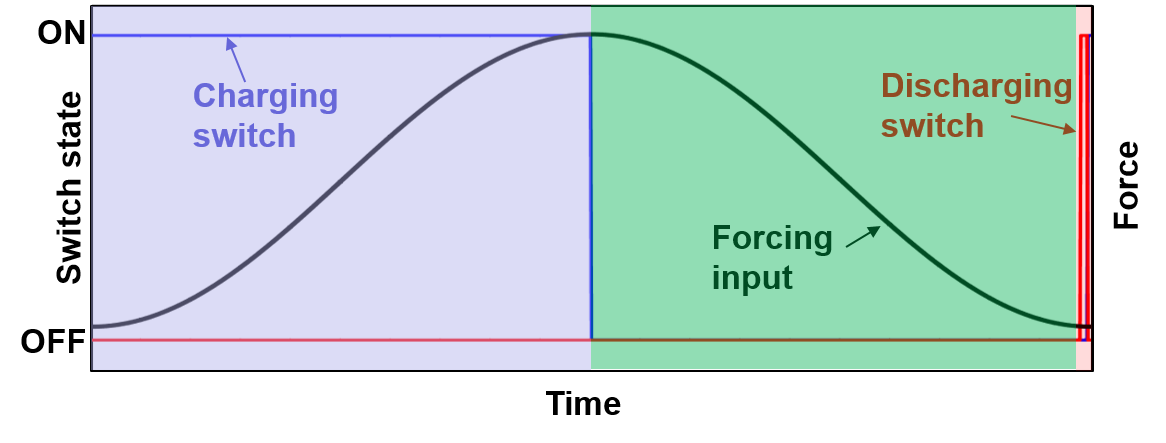
\includegraphics[height=3cm]{Fxt_Cycle.png}
   \end{tabular}
   \end{center}
   \caption[example] 
%>>>> use \label inside caption to get Fig. number with \ref{}
   { \label{fig:FandSW} 
Switch state during the DEG cycle: the charging switch (S1) is kept on while the DEG stretches (blue), both switches (S1 and S2) are off during the relaxing phase (green), and the discharging switch (S2) turns on briefly at the end of the relaxing phase (red).}
   \end{figure} 

\subsection{Self-sensing algorithm}
In the \emph{charging phase}, we chose to use the DEA self-sensing method developed by Rizzello et.\ al.\cite{RizzelloSS_improv} since it consists of a simple recursive method to obtain the capacitance, and does not require extra hardware, only the need to sense voltage and current. 
When we apply it to a DEG, it can be directly incorporated in its charging-while-stretching phase. It consists of a Recursive Least Squares (RLS) regression over the difference equation:
\begin{equation} \label{eqn:difSS}
V_k - V_{k-1} = R(i_k-i_{k-1})+\frac{K_\text{T}}{C}(i_k+i_{k-1}),
\end{equation}
which is obtained from the state space model considering electrode resistance, while neglecting the leakage resistance (since its has practically no effects at high frequencies). $K_\text{T} = \text{tan}(\pi f_\text{e}/f_\text{s})/2\pi f_\text{e}$, with $f_\text{e}$ being the frequency of the sinusoidal sensing signal used and $f_\text{s}$ the sampling frequency used. In \cref{eqn:difSS}, $V$ denotes the measured voltage, $R$ the equivalent resistance of the electrodes and contacts in series with the DE, $C$ the DE capacitance and $i$ the measured current through the DE, while subscripts $k$,  $k-1$ refer to the sample number. 

In the \emph{relaxing phase}, we have open-circuit condition, meaning there is no current flowing in or out of the DEG. Here, the charge in the DEG can be estimated by
\begin{equation}\label{eqn:ph2}
C_k = V_k^{-1}C_{k-1}V_{k-1}\exp\left(-\frac{t_k - t_{k-1}}{R_\text{l}C}\right),
\end{equation}
where $t$ is the sampled time, and $R_\text{l}C$ is assumed constant since, as $C$ decreases, $R_l$ increases at the same rate\cite{RN686}. This assumption allows us to measure (and retain) the values of $R_\text{l}$ and $C$ at the start of the relaxing phase.

During the \emph{discharge phase}, we have high current flowing from the DEG and proportionally low charge, meaning the discharge interval is short when compared to the overall cycle. Thus, assuming that the capacitance remains constant is a reasonable approach. So for the third phase, we simply assume that
\begin{equation}\label{eqn:ph3}
C_{k}=C_{k-1}.
\end{equation}

Alternating the models described above, in accordance with the states of the switches S1 and S2, we estimate the capacitance of the DEG using \ref{eqn:difSS,eqn:ph2,eqn:ph3}. This novel combined self-sensor and DEG shows good agreement between true and self-sensed capacitance, as shown in \ref{fig:capacitance}. To further improve capacitance estimation accuracy, comb filters can be used to eliminate noise and harmonics around the self-sensing signal frequency. 
\begin{figure} [ht]
   \begin{center}
   \begin{tabular}{c} %% tabular useful for creating an array of images 
   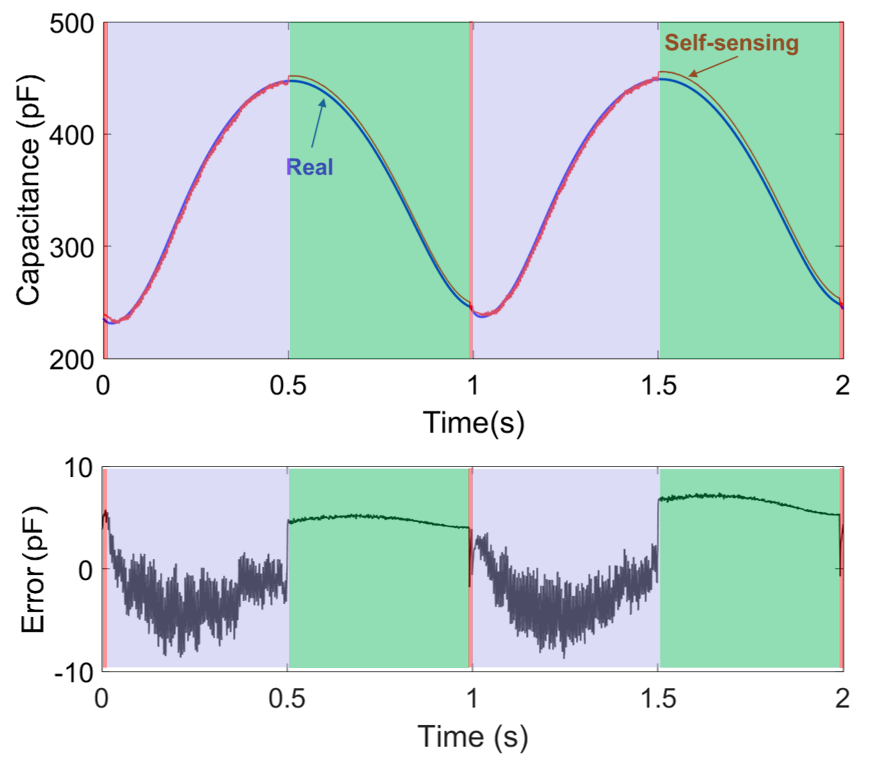
\includegraphics[height=8cm]{Capacitance_sensing.PNG}
   \end{tabular}
   \end{center}
   \caption[example] 
%>>>> use \label inside caption to get Fig. number with \ref{}
   { \label{fig:capacitance} 
(a) Capacitance and (b) error estimated by the self-sensing method during a DEG cycle.}
   \end{figure} 
    
   It is important to note that the higher the amplitude and frequency of the sensing signal, the higher the induced current, and therefore the higher the signal-to-noise ratio, providing better and more reliable values. On the other hand, this also suggests more energy consumed by the self-sensor; a design compromise that must be considered if energy harvesting is the main goal. We point out that, since DEs behave mostly as capacitors, the dissipated power is comparably small with respect to the instantaneous power, as it is mostly reactive\cite{rizzelloOEA}.



\section{CHARGE MANAGEMENT}

As mentioned above, in order to obtain the maximum performance from a DEG, we need to have the charging process completed before the relaxing phase and discharging complete before the DEG starts stretching again. In order to do so, we can extend the self-sensing method, to also identify local maxima and minima in the capacitance signal.
This \emph{peak detection} uses a robust sliding-mode differentiator\cite{Shtessel2014SlidingObservation} to obtain the first and second derivatives of the capacitance signal from the self-sensor. In order to obtain more robust estimation, we used a 5th order differentiator, which provided good results for the first and second derivatives we intend to use. The differentiator is implemented through the set of equations
\begin{align}\label{eq:diff}
\dot{z}_0 &= -\lambda_{k}L^{1/(k+1)}\abs{z_0-C}^{k/(k+1)}\sgn(z_0-C)+z_1,  \nonumber\\
&\vdots \nonumber\\
\dot{z}_j &= -\lambda_{k-j}L^{1/(k-j+1)}\abs{z_{j}-\dot{z}_{j-1}}^{(k-j)/(k-j+1)}\sgn(z_{j}-\dot{z}_{j-1})+z_{j+1}, \\
&\vdots \nonumber\\
\dot{z}_k &= -\lambda_{0}L \sgn(z_{k}-\dot{z}_{k-1}),\nonumber
\end{align}
where $\dot{z_j}$ is the $j$th order derivative estimator, $L$ is the Lipschitz constant\cite{Shtessel2014SlidingObservation}, $\lambda_j>0$ are 
control parameters, and $k$ is the highest order derivative we want to compute. A recursive discrete integration of those derivatives is provided as input to the following step (note $z$ is needed to calculate $\dot{z}$). Thus, our differentiator has seven parameters to be tuned ($\lambda_0,\lambda_1, \ldots, \lambda_5$ and $L$), chosen in order to provide the necessary balance between noise (too high) and delay (too low) in the calculated derivatives. Values of $\lambda_i$ that provided satisfactory results are shown in \cref{tab:parameters} and $L$ can be chosen as a function of the expected mechanical excitation cycle period $T$, e.g.\ $L = 200T$.
\begin{table}[ht]
\caption{Control parameters $\lambda_i$} 
\label{tab:parameters}
\begin{center}       
\begin{tabular}{|l|l|} %% this creates two columns
%% |l|l| to left justify each column entry
%% |c|c| to center each column entry
%% use of \rule[]{}{} below opens up each row
\hline
\rule[-1ex]{0pt}{3.5ex}  $\lambda_0$ & 1.5  \\
\hline
\rule[-1ex]{0pt}{3.5ex}  $\lambda_1$ & 5  \\
\hline
\rule[-1ex]{0pt}{3.5ex}  $\lambda_2$ & 8  \\
\hline
\rule[-1ex]{0pt}{3.5ex}  $\lambda_3$ & 12  \\
\hline
\rule[-1ex]{0pt}{3.5ex}  $\lambda_4$ & 18  \\
\hline
\rule[-1ex]{0pt}{3.5ex}  $\lambda_5$ & 150  \\
\hline
\end{tabular}
\end{center}
\end{table} 
Since noise might still exist, we filter the derivative signals of interest (here, first and second) using low pass filters setting its parameters based on the expected bandwidth of the mechanical excitation of the dielectric elastomer.

To find a local maximum, we seek states which satisfy the following four conditions:
\begin{enumerate}
\item $\sgn(\dot{C}_k)\neq \sgn(\dot{C}_{k-1})$,
\item $ C_k  < C_{k-1}$,
\item $\langle\ddot{C}\rangle<0$,
\item $C_k>(1+x)C_\text{min}$,
\end{enumerate}
where $\dot{C}_k$ is a calculated value of the capacitance's first derivative, $\langle\ddot{C}\rangle$ is the average of the last $N$ values of the second derivative, and $C_\text{min}$ is the capacitance value of the last point that was considered a minimum, corrected by a forgetting factor $x$. Condition 1 provides the basis for a maximum detection, since it represents the change of sign of the first derivative. Conditions 2 and 3 seek to guarantee that the capacitance is decreasing (after it reaches a maximum). Condition 4 aims to add robustness and avoid noise or small perturbations, since charge/discharge of the material might provide small variations in capacitance due to the electrostatic pressure from the charges, rather than the external forcing of the DEG across a cycle that we wish to identify. In order to account for change of circumstances where the cycle amplitude is reduced, we apply a forgetting factor that multiplies and corrects $C_\text{min}$ at each step of the controller, progressively reducing it and making peak detection more likely. To detect a local minimum, the conditions 1--4 above are inverted accordingly.

\section{RESULTS}

In order to validate the new proposed Self-Sensing with Peak Detection (SSPD) method, we tested it in simulation, using validated DE models\cite{RN702}. Measurement noise is also emulated in current and voltage signals of the same order of magnitude as found in realistic measurement devices. This permits to validate the robustness of the method in realistic operating conditions. The SSPD was successfully able to sense the displacement, detect the maxima and minima and promote charging/discharging when we simulated random DEG displacements,as shown in \cref{fig:random}. This demonstrates its potential to be implemented in systems where amplitude and frequency of DEG excitation are unknown, such as generation plans\cite{RN21,RN210,RN164}. Moreover, in order to analyze the bandwidth of the SSPD, it was also tested with varying excitation frequency, as shown in \cref{fig:sweep}. As frequency increases, we have a reduction in the accuracy of our detection. Such errors are a consequence of the filtering techniques, which promote delay in the sensing signal. Such parameters are yet to be optimized, but information on the expected range of frequencies should allow a better choice.

\begin{figure} [ht]
   \begin{center}
   \begin{tabular}{c} %% tabular useful for creating an array of images 
   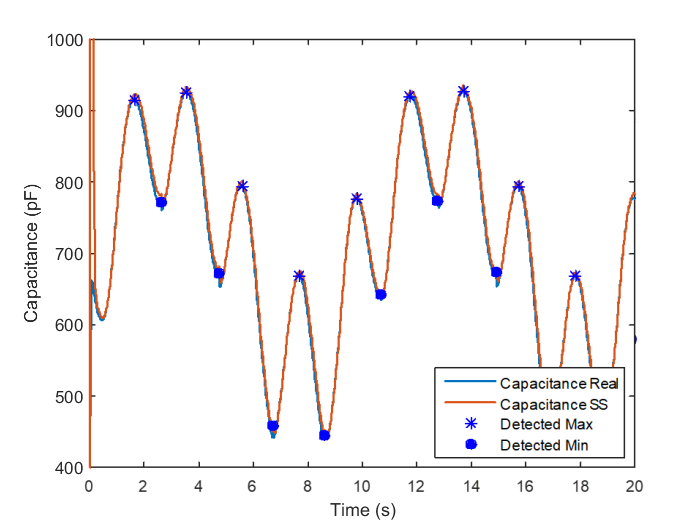
\includegraphics[height=8cm]{random2.png}
   \end{tabular}
   \end{center}
   \caption[example] 
%>>>> use \label inside caption to get Fig. number with \ref{}
   { \label{fig:random} 
Capacitance (pF) as a function of time, together with the results obtained through the  Self-sensing with Peak Detection method, when a DEG subjected to random excitation signal.}   \end{figure} 
   
   \begin{figure} [ht]
   \begin{center}
   \begin{tabular}{c} %% tabular useful for creating an array of images 
   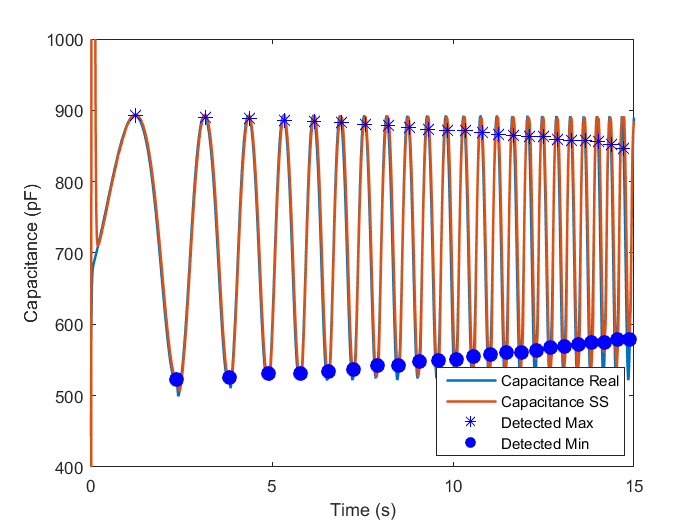
\includegraphics[height=8cm]{SSPD_freq_uniform_displacement.png}
   \end{tabular}
   \end{center}
   \caption[example] 
%>>>> use \label inside caption to get Fig. number with \ref{}
   { \label{fig:sweep} 
Capacitance (pF) as a function of time and the results obtained through the peak detection algorithm and self-sensing when a DEG subjected to excitation frequencies from 0.1Hz to 3Hz.}
   \end{figure}


In order to quantify and compare the efficacy of the SSPD method, we also simulated the same cycle for stable sinusoidal excitation and programmed the charge and discharge to be aligned with the peaks; the ideal scenario that gives the best performance. As illustrated in \cref{fig:er_sweep}, the error in the peak detection increases as the frequency increases, due to the filtering delay (as explained above), but it also shows how error might increase as frequency reduces. The explanation for such cases is that slower variation in capacitance means smaller absolute values in the first and second derivatives that are used by the SSPD. As the noise level is kept constant, higher noise-to-signal ratio leads to an early peak detection, as the zero-crossing in the first derivative happens earlier due to the noise. 
When we compare the energy harvesting performance, as shown in \cref{fig:en_sweep}, we see the price of the inaccuracy for higher frequency: the delayed peak detection reduces the useful capacitance swing in the cycle, thus reducing the energy harvested. Further, since we spend energy in the self-sensing process, lower frequency also reduces the final amount of energy harvested. Nevertheless, the proposed method allows us to autonomously run and repeat the desired cycle independent of quantitative knowledge of external excitations and without the need of further sensors.
  
   
   
   \begin{figure} [ht]
   \begin{center}
   \begin{tabular}{c} %% tabular useful for creating an array of images 
   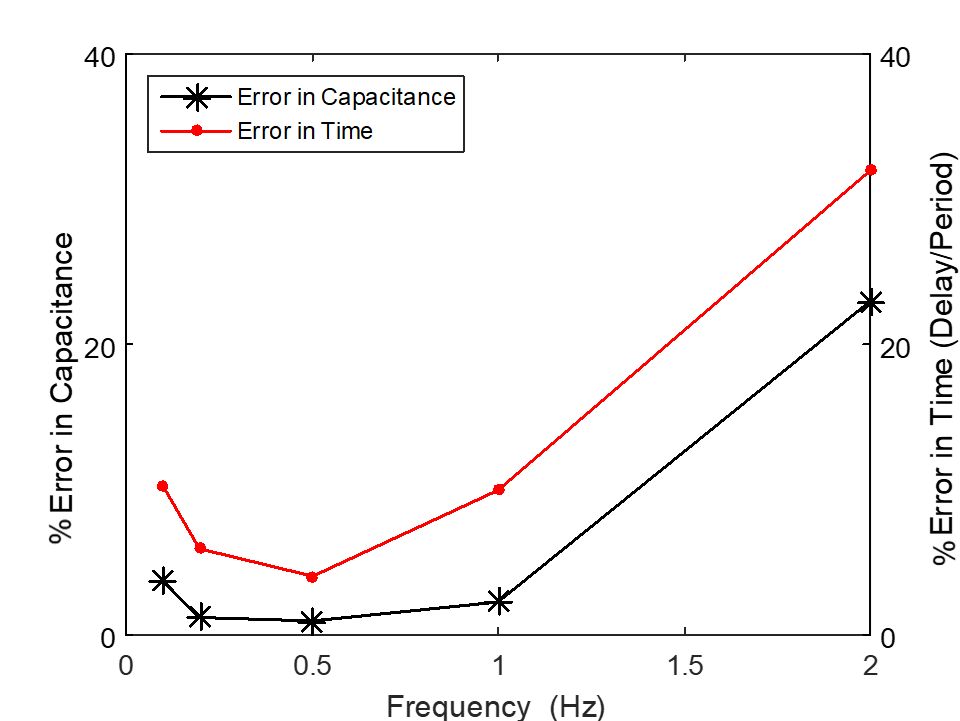
\includegraphics[height=8cm]{error_sweep2.png}
   \end{tabular}
   \end{center}
   \caption[example] 
%>>>> use \label inside caption to get Fig. number with \ref{}
   { \label{fig:er_sweep} 
Errors in the peak detection algorithm for different frequencies.}
   \end{figure}   
   
   \begin{figure} [ht]
   \begin{center}
   \begin{tabular}{c} %% tabular useful for creating an array of images 
   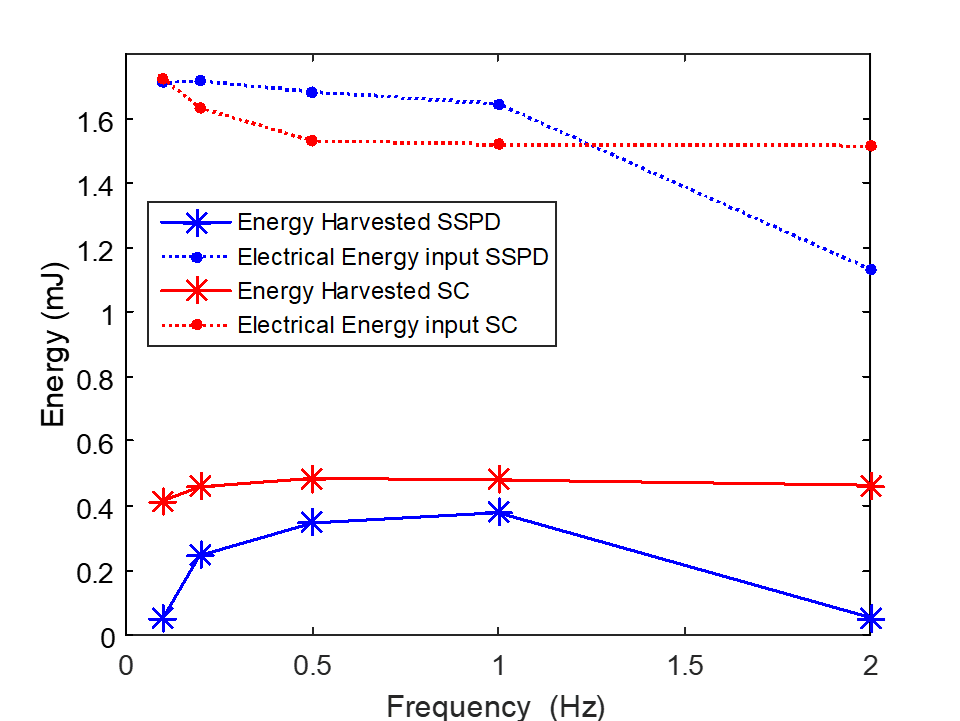
\includegraphics[height=8cm]{energy_sweep.png}
   \end{tabular}
   \end{center}
   \caption[example] 
%>>>> use \label inside caption to get Fig. number with \ref{}
   { \label{fig:en_sweep} 
 Energy input and harvested comparing the peak detection algorithm (SSPD) with a Scheduled Charge/Discharge (SC) for a known sinusoidal deformation for different frequencies.}
   \end{figure}   
   
   


\section{CONCLUSION}

In this paper, we have reported the development of a new method to automatically manage the charging  and discharging process in DEGs through the use of an integrated self-sensing and peak detection (SSPD) algorithm. The method is able to perform without knowledge of the external load, thus requiring only a microprocessing unit and voltage/current sensors (which are expected to be integrated in DEG energy generation setups for monitoring). Further work includes the practical implementation to verify the hardware processing speeds that are necessary. In addition, SSPD performance can be further increased by the optimization of its parameters and filters, adapted to a chosen application. 
